%!TEX root = ../main.tex

\chapter{Related Works}
\label{chp:related}

Performing federated analytics tasks requires a robust architecture composed by different layers: a federation layer that allows for multiple streaming connections with diverse and heterogeneous sources (relational, no-SQL and columnar \ac{DBMS}s); a virtualization layer that exposes "virtual" relational views of non-materialized data; an integration, ontology-based layer, so to add a semantic layer to the virtualized relational views, given the importance of exploring complex relationships among genomics data.

This approach has been formalized under the concept of \ac{OBDF} \cite{DBLP:conf/icde/GuCPLMX24}, and it is represented in Fig. \ref{fig:obdf}. As far as we know, no existing off-the-shelf system implementing this framework has ever been released: who intends to apply this architecture design have to manually install different components choosing among diverse competitors, and combining them together, dealing with possible underlying platform incompatibilities. Moreover, having no off-the-shelf solutions implies having no solutions specifically tailored and optimized for dealing with genomics data.

\begin{figure}[ht]
    \centering
    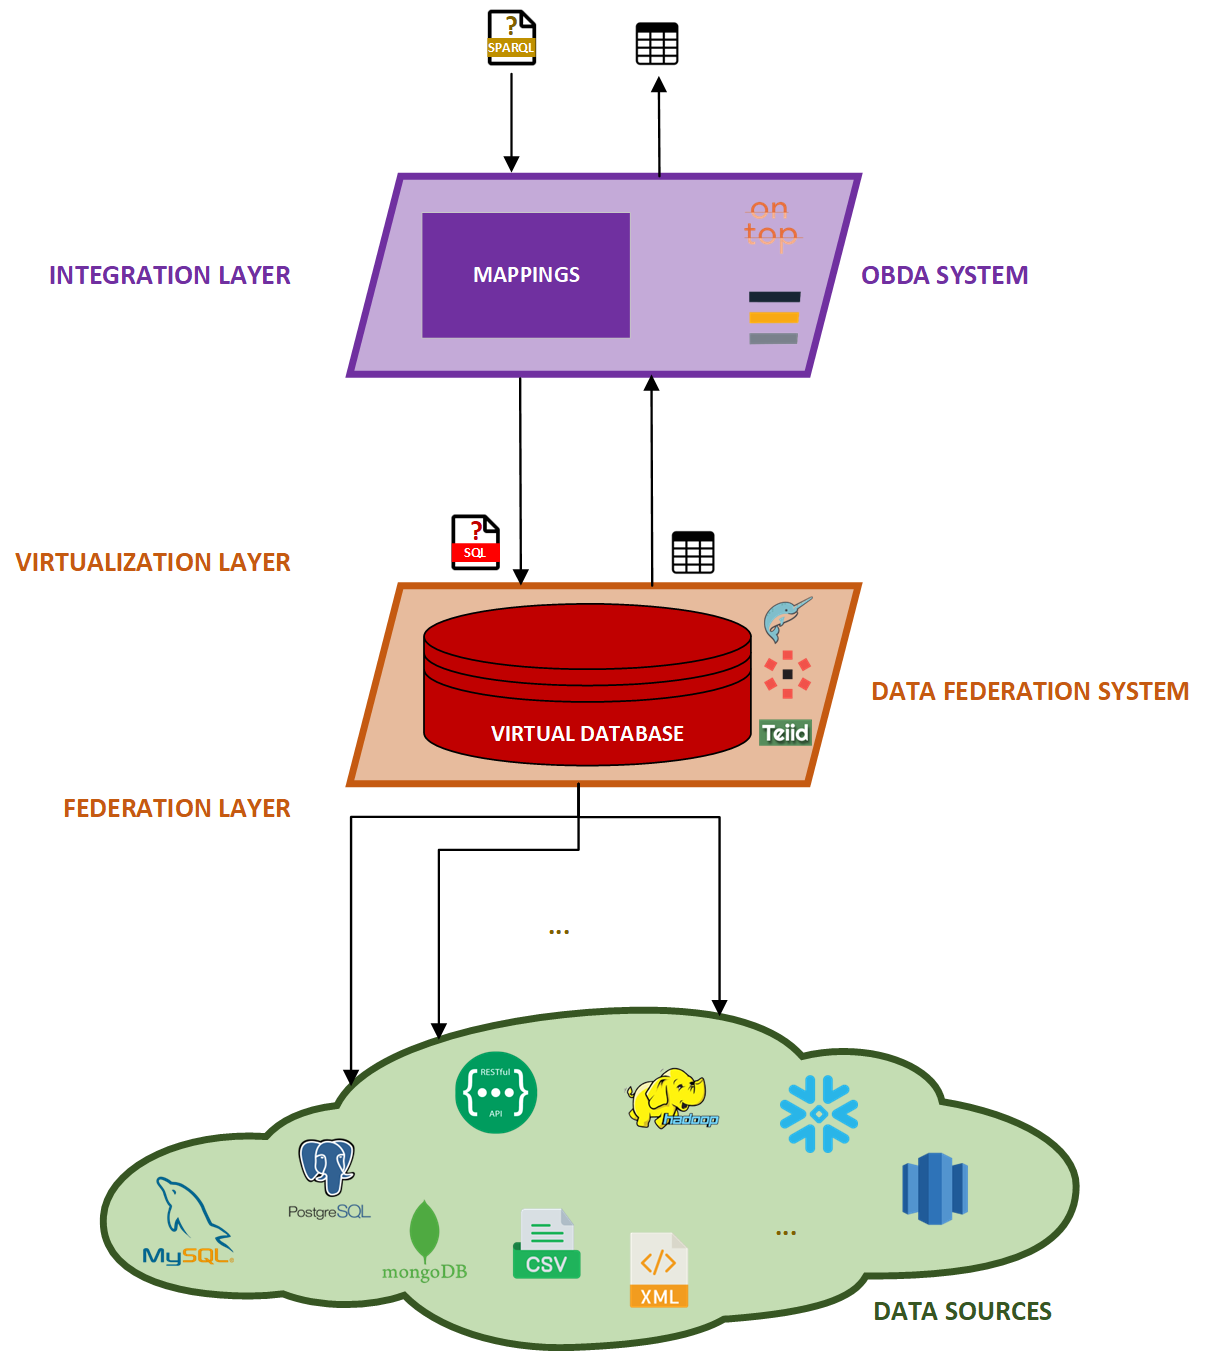
\includegraphics[width=11.5cm]{res/Drawing4.png}
    \caption{OBDF approach}
    \label{fig:obdf}
\end{figure}

Nonetheless, similar design proposal have been implemented in order to address both research questions as well as enterprise requirements. In this section, we will briefly discuss two solutions, one for each environment, analyzing them in details, highlighting strengths and weaknesses.

\section{BigDAWG}
\ac{BigDAWG} \cite{DBLP:conf/hpec/GadepallyCDEHKM16} represents a crucial milestone in the world of polystore systems, designed to address the complexities of managing heterogeneous data environments. Developed under at the Intel Science and Technology Center for Big Data, \ac{BigDAWG}'s architecture realizes the paradigm "one size does not fit all" in database management systems. This polystore system is engineered to support a wide set of data models and storage engines, offering a unified platform for cross-storage-system queries, real-time analytics, and complex data visualizations.
\subsection{Architecture Overview}
\ac{BigDAWG}'s architecture is meticulously structured into four primary layers: the base layer, the island layer, the main \ac{BigDAWG} layer, and the application layer. Each of these layers serves a distinct function, creating a cohesive system capable of managing diverse data stores and facilitating seamless user interaction through applications.
\subsubsection{Base Layer}
The base layer of \ac{BigDAWG} consists of the physical data stores, which include a variety of storage engines such as relational databases (e.g., PostgreSQL), array databases (e.g., SciDB), key-value stores (e.g., Apache Accumulo), and streaming databases (e.g., S-Store). Each of these storage systems is optimized for  specific types of data and query workloads, adhering to the principle that no single storage engine is best suited for all types of data. This layer is responsible for the actual storage and retrieval of data, leveraging the strengths of each specialized engine to handle the respective data types effectively.
\subsubsection{Island Layer}
Above the base layer is the island layer, a critical abstraction within \ac{BigDAWG}'s architecture. An "island" in \ac{BigDAWG} represents a domain-specific environment tailored to a particular data model and query language. For example, the relational island interfaces with traditional RDBMSs like PostgreSQL, the array island interacts with SciDB, and the text island is linked to systems like Accumulo. Each island encapsulates the syntax and semantics of its underlying data model, thus preserving the rich functionalities and optimizations offered by the native storage engines. The island layer also facilitates the casting of data between different islands, enabling queries that span multiple data models. The ability to perform these cross-island operations is central to \ac{BigDAWG}’s polystore capability, ensuring that users can execute queries that utilize the most appropriate data model for each part of their analysis.
\subsubsection{Main BigDAWG Layer}
The main \ac{BigDAWG} layer orchestrates the interaction between the various islands and the underlying data stores. This layer includes components such as the query planner, optimizer, and the casting engine, which collectively manage the distribution of queries across the appropriate islands. The casting engine is particularly noteworthy, as it enables the movement of data between different storage systems, translating data formats and query languages as needed. For instance, data stored in an array database might be cast into a relational format to allow for SQL-based analytics, and then cast back into an array format for further processing.
This layer is also responsible for maintaining metadata about the data stores and islands, including information about data distribution, query capabilities, and performance characteristics of each storage engine. This metadata is crucial for optimizing query execution, as it allows \ac{BigDAWG} to intelligently route queries to the most suitable storage engine based on the query's requirements and the data's location.
\subsubsection{Application Layer}
At the top of the \ac{BigDAWG} architecture is the application layer, which provides user-facing tools and interfaces for interacting with the system. This layer includes APIs for query submission, tools for data visualization, and interfaces for real-time data monitoring and complex analytics. \ac{BigDAWG} supports a variety of applications, from simple SQL-based data retrievals to complex analytics involving machine learning and real-time data processing. The application layer abstracts the underlying complexity of the polystore system, offering a unified interface that allows users to focus on their data analysis tasks without needing to understand the intricacies of the underlying data storage systems.
\subsection{Operational Principles and Innovations}
\ac{BigDAWG}'s operational principles are grounded in the concept of federating multiple, heterogeneous data stores while preserving the specialized capabilities of each storage engine. This approach allows \ac{BigDAWG} to offer a robust platform for executing complex queries across different data models, something that traditional database systems struggle to achieve.
\subsubsection{Islands and Cross-Island Querying}
The island-based architecture is one of \ac{BigDAWG}'s most significant innovations. By organizing data stores into islands, \ac{BigDAWG} allows users to interact with data using the most appropriate data model and query language. This capability is particularly important in environments where data is stored in multiple formats, each optimized for a different type of analysis. For example, a user might store time-series data in an array database like SciDB while storing text data in a key-value store like Accumulo. \ac{BigDAWG}'s island architecture allows the user to query both datasets in a single operation, casting the results into a common format for further analysis.
The cross-island query capability is facilitated by the casting engine, which can translate data formats and query languages on-the-fly. This ensures that data can be moved between islands without loss of fidelity or functionality. For instance, a query might start in the relational island to extract patient metadata from PostgreSQL, then cast the data into the array island to perform complex mathematical operations on waveform data stored in SciDB, and finally cast the results back into the relational island for final aggregation and reporting.
\subsubsection{Performance Optimization}
Another key feature of \ac{BigDAWG} is its ability to optimize query performance \cite{DBLP:conf/hpec/SheRD16} by leveraging the strengths of the underlying storage engines. The system's query planner uses metadata about the data stores and islands to determine the most efficient way to execute a query. For example, if a query involves a large text search, \ac{BigDAWG} might choose to cast the data into the text island, where the key-value store (e.g., Accumulo) can handle the search more efficiently than a relational database. Similarly, if the query involves complex mathematical operations on large datasets, the planner might route the query to the array island, where SciDB's array-based storage engine can perform the operations more efficiently.
\ac{BigDAWG} also supports real-time data processing, making it suitable for applications that require immediate responses, such as monitoring systems in healthcare settings. The system's streaming capabilities, provided by engines like S-Store, allow it to handle high-velocity data streams while maintaining transactional consistency. This is particularly important in environments like medical data monitoring, where delays or errors in data processing could have serious consequences.
\subsubsection{Use Cases and Practical Implementations}
\ac{BigDAWG} has been demonstrated in several complex real-world scenarios \cite{DBLP:journals/pvldb/ElmoreDSBCGHHKK15} \cite{DBLP:conf/vldb/Mucklo18}, highlighting its versatility and robustness. One of the most prominent use cases is the management of the MIMIC II dataset, a large-scale medical database containing various types of data, including time-series waveform data, patient metadata, and clinical notes.
\subsubsection{MIMIC II Dataset Management}
The MIMIC II dataset is a prime example of a heterogeneous data environment, where different types of data require different storage and processing techniques. \ac{BigDAWG} effectively manages this dataset by distributing the data across multiple storage engines, each optimized for a specific type of data. For instance, patient metadata is stored in PostgreSQL (relational island), waveform data is stored in SciDB (array island), and clinical notes are stored in Accumulo (text island). \ac{BigDAWG}'s ability to perform cross-island queries allows researchers to analyze the data in a holistic manner, combining insights from the different data types into a single analysis.
In practical terms, this means that a query might involve extracting patient metadata from PostgreSQL, performing a Fourier transform on the waveform data in SciDB, and searching for relevant clinical notes in Accumulo. \ac{BigDAWG} handles the complex task of routing the query through the appropriate islands, casting the data as needed, and optimizing the execution to minimize processing time and resource usage. This capability is particularly valuable in medical research, where researchers need to quickly and accurately analyze large datasets to draw meaningful conclusions.
\subsubsection{Challenges and Future Directions}
Despite its advanced architecture and capabilities, \ac{BigDAWG} is not without challenges. One of the main issues is its prototype nature; it is not available as an off-the-shelf solution and requires significant expertise to install, configure, and extend. This limits its accessibility to organizations with the necessary technical skills and resources. Furthermore, the development of new islands to support additional data models and storage engines requires a deep understanding of both the \ac{BigDAWG} system and the underlying technologies.
Another challenge is the limited literature and empirical studies on \ac{BigDAWG}'s deployment in real-world scenarios. While the system has been successfully demonstrated in academic and research environments, there is still a lack of comprehensive studies on its performance and reliability in operational settings. This raises questions about its scalability and robustness when applied to large-scale, production environments.
\subsection{Conclusion and Future Work}
In conclusion, \ac{BigDAWG} represents a significant advancement in the field of polystore systems and heterogeneous data management. Its multi-layered architecture, island-based abstraction, and cross-island querying capabilities offer a powerful solution for managing and analyzing complex datasets. However, its practical application is currently limited by the need for specialized knowledge and the lack of extensive real-world testing.
Future research could focus on several key areas to reduce the barriers to adoption and expand \ac{BigDAWG}'s applicability. These include the development of more user-friendly installation and configuration tools, the creation of additional islands to support a wider range of data models, and the conducting of large-scale empirical studies to validate the system's performance and reliability in operational environments. Additionally, efforts could be made to improve the system's documentation and provide more comprehensive training resources to help users understand and leverage its full capabilities.

\section{Optique}
The Optique system, born from the EU-funded Seventh Framework Programme \cite{DBLP:journals/ijtm/LytrasSP09}, represents a significant evolution in the field of \ac{OBDA} systems tailored for industrial applications \cite{DBLP:conf/semweb/KharlamovBGJLNO15}. Unlike typical OBDA systems which focus predominantly on static data, Optique extends its capabilities to effectively handle both streaming and static data, providing a robust platform designed for real-time and historical data integration and accessibility using semantic technologies. The project involved multiple prestigious institutions and industry giants like Siemens, underscoring a collaborative effort aimed at enhancing data accessibility and integration across varied sectors. Optique documentation relatively to its development stage while project execution is publicly available\footnote{https://mvnrepository.com/artifact/eu.optique-project}.
\subsection{Architectural Overview}
Optique is designed using a layered architecture approach, ensuring scalability and extensibility \cite{DBLP:conf/esws/KharlamovJZBGHHKKORRSSSW13}. At its core, the architecture comprises several distinct layers, each responsible for a specific aspect of the system's functionality:
\begin{itemize}
\item \textbf{Presentation Layer} : This layer includes user interfaces for both end-users and IT experts, facilitating interactions such as query formulation, system configuration, and ontology management. Key interfaces in this layer are developed to ensure user-friendliness and accessibility, allowing users to interact with the system without needing in-depth technical knowledge of the underlying semantic technologies.
\item \textbf{Application Layer}: This layer represents the backbone of the Optique system, hosting critical components including the Query Formulation, Ontology and Mapping Management, and Query Answering components. Each component is designed to handle specific functionalities, from managing ontology mappings to processing complex queries over diverse data sources.
\item \textbf{Data and Resource Layer}: This foundational layer manages the data sources accessed by the system, which may include relational databases, triple stores, and data streams. It also encompasses the infrastructure required to support the extensive computational needs of the system, leveraging cloud technologies to enhance scalability and performance. 
\end{itemize}
\subsection{Core Components and Functionalities}
The Optique system incorporates several components that improve its performance and usability:
\subsubsection{STARQL Query Language}
At the heart of Optique's functionality is STARQL, an advanced query language that enables complex querying over both streaming and static data. STARQL supports seamless integration of streaming data queries, allowing for real-time data processing and analytics.
\subsubsection{ExaStream Backend System}
ExaStream represents the backend processing component of Optique, optimized for handling high-velocity data streams with minimal latency. Its design focuses on efficient data ingestion and query processing, ensuring that the system can manage the continuous influx of data from industrial sensors and other real-time data sources.
\subsubsection{OptiqueVQS: Visual Query System}
The Optique Visual Query System (OptiqueVQS) enhances the accessibility of the system by enabling users to construct queries visually \cite{DBLP:journals/semweb/SoyluKZJGSHSBLH18}. This component is particularly useful for users without experience in query languages, as it provides an intuitive interface for building and executing queries, and thus reducing dependence on IT departments and streamlining data access processes.
\subsection{Impact and Evaluation}
The deployment of Optique has shown a scalable approach to data access, significantly reducing the reliance on IT intermediation and promoting efficient data utilization. 
However, despite its advanced capabilities, the integration of Optique within the Siemens ecosystem has led to its status as a proprietary system. This exclusivity could potentially restrict broader adoption and external validation, posing challenges in comparative analyses against other OBDA systems in diverse real-world settings.